\documentclass[]{standalone}
\usepackage{mathptmx}
%\renewcommand{\familydefault}{\rmdefault}
\usepackage[T1]{fontenc}
\usepackage[latin9]{inputenc}
\usepackage{siunitx}
\usepackage{array}
\usepackage{amsmath}
\usepackage{ifthen}
\usepackage{pgfplots}
\pgfplotsset{compat=1.14}
\usepackage{titling, graphicx}
\usepackage{tikz}
\usepackage{upgreek}
\usepackage{amsmath,amsthm}
\usepackage{strtikz}
\usetikzlibrary{shapes,arrows.meta,intersections,graphs,graphs.standard,math,fit}
\usetikzlibrary{calc,intersections,through,backgrounds}
\usetikzlibrary{decorations.pathmorphing, decorations.markings,decorations.pathreplacing}


\begin{document}
\def \fsize {\footnotesize}
\begin{tikzpicture}
\bilinear[startx = 0cm,
starty = 0cm,
yield displacement = 0.5cm,
yield force = 2cm,
maximum displacement = 4cm,
maximum force = 2.5cm,
axis space = 0.5cm,
mode = 4,
x-axis label = \fsize {Rotation},
y-axis label = \fsize {Moment},
kp text = \fsize $k_\text{p}$,
ks text = \fsize $k_\textrm{s}$,
fy text = \fsize $M_\textrm{y}$,
dy text = \fsize $\theta_\textrm{y}$,
mark yield point = 1,
fmax text = \fsize $M_\textrm{m}$,
dmax text = \fsize $\theta_\textrm{m}$,
mark max point = 0]
%\draw (0,0) -- (1cm,1cm);
\end{tikzpicture}
\end{document}